\chapter{Logical View}
The logical view represents the classes and the objects of the system. Since we don't want
to dig too specific into the class structure of the different components, we will show some
diagrams of a higher level of the system. The diagrams show how the different subsystems
are related to each other, how they are connected with each other and also how they evolve
as the system evolves into it's final form.


%info over Logical viewpoint
\section{Information}
In this view, we want to show the way in which the system evolves from the current situation into 
the desired situation where both companies are merged, we first have to give a graphical 
representation of the current system. From here on, we improve the system in certain steps to
make the system more modular and changeable. To show these changes, we decided to point out 
three deadlines, at which we expect that the system is adapted according to this document.
These deadlines will be addressed to as \emph{Phase 1}, \emph{Phase 2} and \emph{Phase 3}\\
 \\
We also think that at each phase, the system will be still fully functional and working correctly.
The whole architecture is set up in a way that all the functionality of the prior phase, will still 
be available at the end of the phase. If -for instance in the case of STIFF- it wasn't possible to 
refactor the whole application in the first phase, but we did want to provide on-demand calculations,
we designed a wrapper around the system to provide this functionality as soon as possible.
The wrapper will be removed when we refactor the STIFF system, but now with little effort, we can
keep the functionality of the system as a whole intact.\\
 \\
The figures in this view show the modularity of the system. Every subsystem has its own
functionality, which makes it easy to make changes to one of the subsystems separately.
Because of this modularity, the testability and the changeability of the system is also good.



\section{The current system}
The current system consists of several smaller programs which interact with each other. 
The following components are identified in the current architecture: 
\begin{itemize}
\item UCIS: Universal Customer Information System
\item ProD: Product Database
\item STIFF: System for Tariff Information For Fee-calculations
\item ProFi: Proposal Financials
\item Print Proposals
\item CHIPS: Claim Handling and Payment System
\item BuRP: Bulk Refund Product
\end{itemize}
For more detailed information of these systems, we would like to point to the spe\-ci\-fi\-ca\-tions
given in the Request for Architecture of the SureThing company

\subsubsection{Logical View}
Below you see the logical representation of the current system.
\begin{figure}[ht]
	\centering
		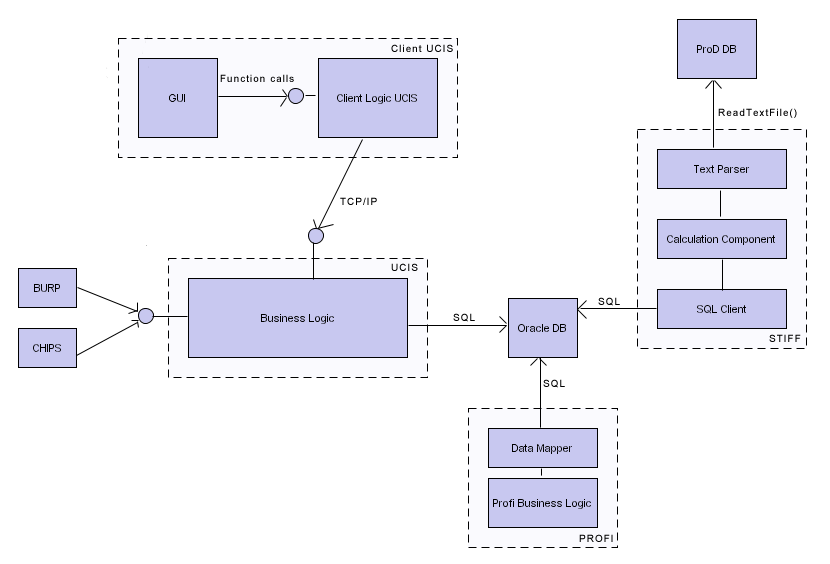
\includegraphics[width=1.00\textwidth]{img/logical-current.png}
	\caption{Image of the current system}
	\label{fig:logical-current}
\end{figure}

\subsubsection{Additional information}
As you see in the picture, the current system provides two databases, one for the product
information, and one for the customer information. Since the ProD is a plain-text database,
it is desirable to move this information into the main (relational) database. The current 
STIFF system is also fairly outdated. It is written in COBOL, which makes changing this
application very hard. The system also cannot provide real-time calculations of proposals
to the UCIS system. All the calculations are currently done in batch-mode at midnight.\\
The client software has gained more and more logic into its components. These calculations
should be incorporated in the business logic at the UCIS server component. In the most 
desirable case, we want the client software only to be able to display the Graphical User 
Interface, and the client software should not have any logic implemented at all.\\
 \\
The matter in which the changes should be scheduled and applied to the system are addressed
in the following sections.



\section{The system at Phase 1}
In the first iteration we want the STIFF system to behave as a real-time component. 
Because we will not make any big changes to the STIFF logic yet, we decided to make an extra
wrapper around the STIFF system, which starts the calculations on request. The calculations
(and reading of the text-based ProD) are still the same, the only improvement here is that
the calculations are no longer done in batch mode, but real-time and on demand.

\subsubsection{Logical View}
Below you see the logical representation of the system at Phase 1. See figure \ref{fig:logical_phase1}
\begin{figure}[ht]
	\centering
		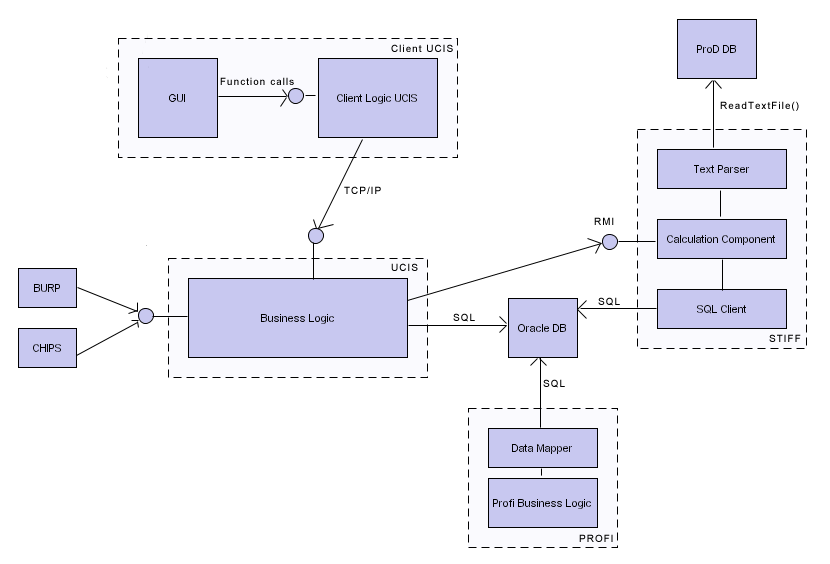
\includegraphics[width=1.00\textwidth]{img/logical-phase1.png}
	\caption{Logical View after phase 1}
	\label{fig:logical_phase1}
\end{figure}

\subsubsection{Additional information}
We choose to use RMI as the interface to the STIFF component, because it makes the implementation
more easy. With Java RMI you don't have to worry about creating sockets for the connections,
because this is already implemented in the RMI specification. The serializing of the objects 
and the object relations is also easier to implement using RMI.



\section{The system at Phase 2}
In the second phase of the system we will mainly refactor the business logic of UCIS.
When we refactor the components, we also have to make CHIPS and BuRP make use of the new
UCIS components that are available.\\
The other main change is that we transform the Graphical User Interface (GUI) of the old
UCIS system into a JSP website.

\subsubsection{Logical View}
Below you see the logical representation of the system at Phase 2. See figure \ref{fig:logical_phase2}
\begin{figure}[ht]
	\centering
		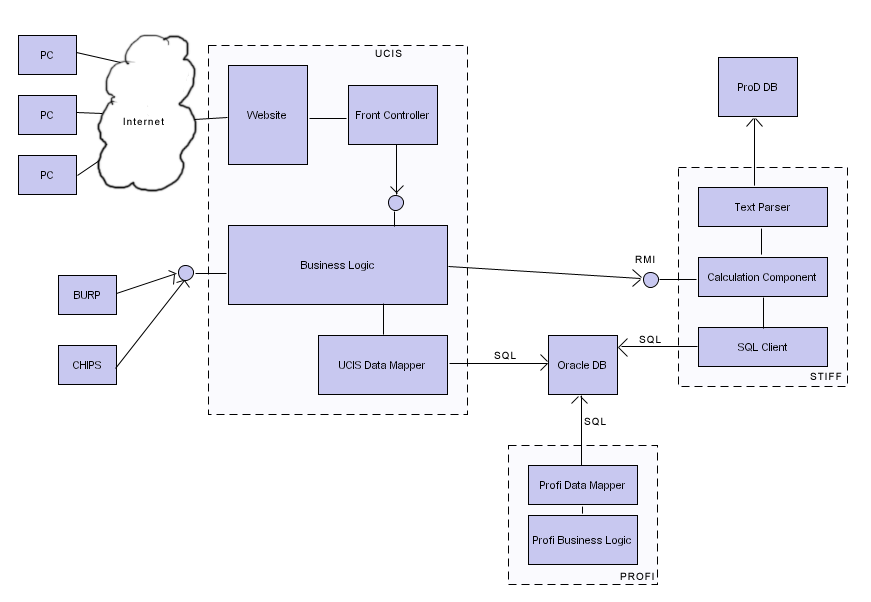
\includegraphics[width=1.00\textwidth]{img/logical-phase2.png}
	\caption{Logical View after phase 2}
	\label{fig:logical_phase2}
\end{figure}


\subsubsection{Additional information}
The main transformation in this phase involves UCIS. This system is refactored to conform to the
layered architecture. All the business logic will be moved to the Business Layer and the the 
Data Mapper will be implemented in the Data Layer. As presentation layer we will use a JSP 
website, which is served to customers through the web server and the Internet. Because of this,
anyone with a web-browser installed on their computer will be able to calculate their own 
proposal. (Access to detailed customer information is restricted of course).\\ 
 \\
The BuRP and CHIPS components do also have to be updated, in a way that they will from now on
use the interface that UCIS provides to get the desired functionality for these systems.



\section{The system at Phase 3}
In the last phase we will refactor the whole STIFF component in Java. A notification system
will be introduced in STIFF, and UCIS has to make use of this notifier at the end of this
phase. The Product Database will also be migrated into the Oracle Database from here on.\\
In this last step we also include the Generic Output Controller (GOC).

\subsubsection{Logical View}
Below you see the logical representation of the system at Phase 3. See figure \ref{fig:logical_final}
\begin{figure}[ht]
	\centering
		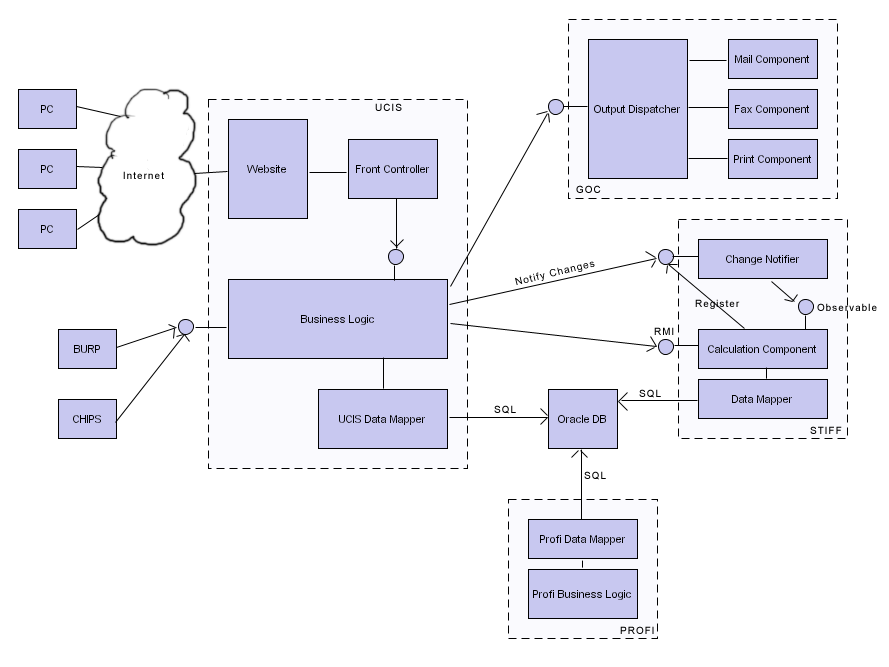
\includegraphics[width=1.00\textwidth]{img/logical-final.png}
	\caption{Logical View for final system}
	\label{fig:logical_final}
\end{figure}


\subsubsection{Additional information}
The whole STIFF component will be refactored in Java. The old system of STIFF was
completely written in COBOL, which made it very hard to make changes in. To provide 
real-time proposal calculations, the system had to be scalable to some extent. We can 
only make STIFF scalable, if we refactor it completely to Java.\\
The calculations that have to be calculated in real-time, take a lot of resources of the 
STIFF system. To ensure real-time calculations of the proposals, we have to make the STIFF 
component scalable. That means, that is the load on the server becomes to high, we can add 
another server to STIFF, so that from that point on the load is distributed among the two 
servers. If the amount of requests still grows and more servers are needed, new servers 
can be easily added to the system.\\
 \\
Because of the fact that the product information doesn't change very often, it is not
desirable that each STIFF server requests the latest product information from the database at
each calculation request. To decrease network traffic, and to decrease the load on the 
database server, it is best to store this information in the memory of the server,
and only when the product information changes, that the STIFF servers gather the new 
information from the database.
